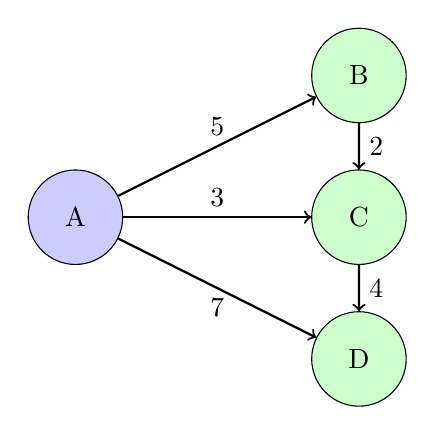
\begin{tikzpicture}[scale=1.2]
  % ノードA
  \node[circle, draw, fill=blue!20, minimum size=1.2cm] (A) at (0,0) {A};
  
  % ノードB, C, D
  \node[circle, draw, fill=green!20, minimum size=1.2cm] (B) at (3,1.5) {B};
  \node[circle, draw, fill=green!20, minimum size=1.2cm] (C) at (3,0) {C};
  \node[circle, draw, fill=green!20, minimum size=1.2cm] (D) at (3,-1.5) {D};
  
  % エッジ
  \draw[->, thick] (A) -- (B) node[midway, above] {5};
  \draw[->, thick] (A) -- (C) node[midway, above] {3};
  \draw[->, thick] (A) -- (D) node[midway, below] {7};
  
  \draw[->, thick] (B) -- (C) node[midway, right] {2};
  \draw[->, thick] (C) -- (D) node[midway, right] {4};
\end{tikzpicture}
